
%\documentclass[mathserif]{beamer}
\documentclass[handout]{beamer}
%\usetheme{Goettingen}
%\usetheme{Warsaw}
\usetheme{Singapore}



%\usetheme{Frankfurt}
%\usetheme{Copenhagen}
%\usetheme{Szeged}
%\usetheme{Montpellier}
%\usetheme{CambridgeUS}
%\usecolortheme{}
%\setbeamercovered{transparent}
\usepackage[english, activeacute]{babel}
\usepackage[utf8]{inputenc}
\usepackage{amsmath, amssymb}
\usepackage{dsfont}
\usepackage{graphics}
\usepackage{cases}
\usepackage{graphicx}
\usepackage{pgf}
\usepackage{epsfig}
\usepackage{amssymb}
\usepackage{multirow}	
\usepackage{amstext}
\usepackage[ruled,vlined,lined]{algorithm2e}
\usepackage{amsmath}
\usepackage{epic}
\usepackage{epsfig}
\usepackage{fontenc}
\usepackage{framed,color}
\usepackage{palatino, url, multicol}
%\algsetup{indent=2em}
\newcommand{\factorial}{\ensuremath{\mbox{\sc Factorial}}}
\newcommand{\BIGOP}[1]{\mathop{\mathchoice%
{\raise-0.22em\hbox{\huge $#1$}}%
{\raise-0.05em\hbox{\Large $#1$}}{\hbox{\large $#1$}}{#1}}}
\newcommand{\bigtimes}{\BIGOP{\times}}
\vspace{-0.5cm}
\title{Natural Language Processing \\ Large Language Models Usage and Evaluation Patterns}
\vspace{-0.5cm}
\author[Felipe Bravo Márquez]{\footnotesize
%\author{\footnotesize  
 \textcolor[rgb]{0.00,0.00,1.00}{Felipe Bravo-Marquez}} 
  
 

\date{\today}

\begin{document}
\begin{frame}
\titlepage


\end{frame}


% Large Language Models (LLMs) have changed the way computers understand and use human language. They're used in many different areas, and in this talk we'll look at how people use and evaluate them. We'll start by looking at the different ways people use LLMs. First, when they are used as general assistants for tasks like writing, summarizing, coding, etc. Then, when they are adapted to address more domain-specific tasks using two approaches: 1) retrieval-assisted generation, and 2) fine-tuning. We'll also see how LLMs are integrated into software applications, such as when they are invoked by computer code (API calls) or used by autonomous agents to make decisions on their own. On the evaluation side, we'll talk about a method called MTBench, a multi-turn question set, and Chatbot Arena, a crowdsourced battle platform between LLMs.





\section{Introduction}
\begin{frame}{Introduction}
\begin{scriptsize}
\begin{itemize}
\item Since the inception of Large Language Models, various patterns of use and evaluation of this technology have emerged.
\item In this talk, we will try to organize these patterns and give a general overview of them.
\end{itemize}

 \begin{figure}[h]
        	
\includegraphics[scale = 0.2]{pics/Large-Language-Models.jpg}
        \end{figure}
Source: \url{https://www.masayume.it/img/masayume/Large-Language-Models.jpg}
\end{scriptsize}
\end{frame}



\begin{frame}{Recap: What is an LLM}
\begin{scriptsize}
\begin{itemize}
\item  Large Language Model: An autoregressive language model trained with a Transformer neural network on a large corpus (hundreds of bullions of tokens) and a large parameter space (billions) to predict the next word.
\item It is usually later aligned to work as a user assistant using techniques such as Reinforcement Learning From Human Feedback  \cite{ouyang2022training} or supervised fine-tuning.
\item Some are private (access via API or web browser): Google Bard, ChatGPT, etc.
\item Others are open (model's weights can be downloaded): Llama, LLama2, Falcon, etc.
\end{itemize}

 \begin{figure}[h]
        	
\includegraphics[scale = 0.4]{pics/gptllama.png}
        \end{figure}

\end{scriptsize}
\end{frame}

\begin{frame}{Zero-shot, One-shot, and Few-shot Learning}
\scriptsize
The most remarkable feature of these models is their few-shot, one-shot, zero-shot learning capabilities (also known as ``in-context-learning'').
 \begin{figure}[h]
        	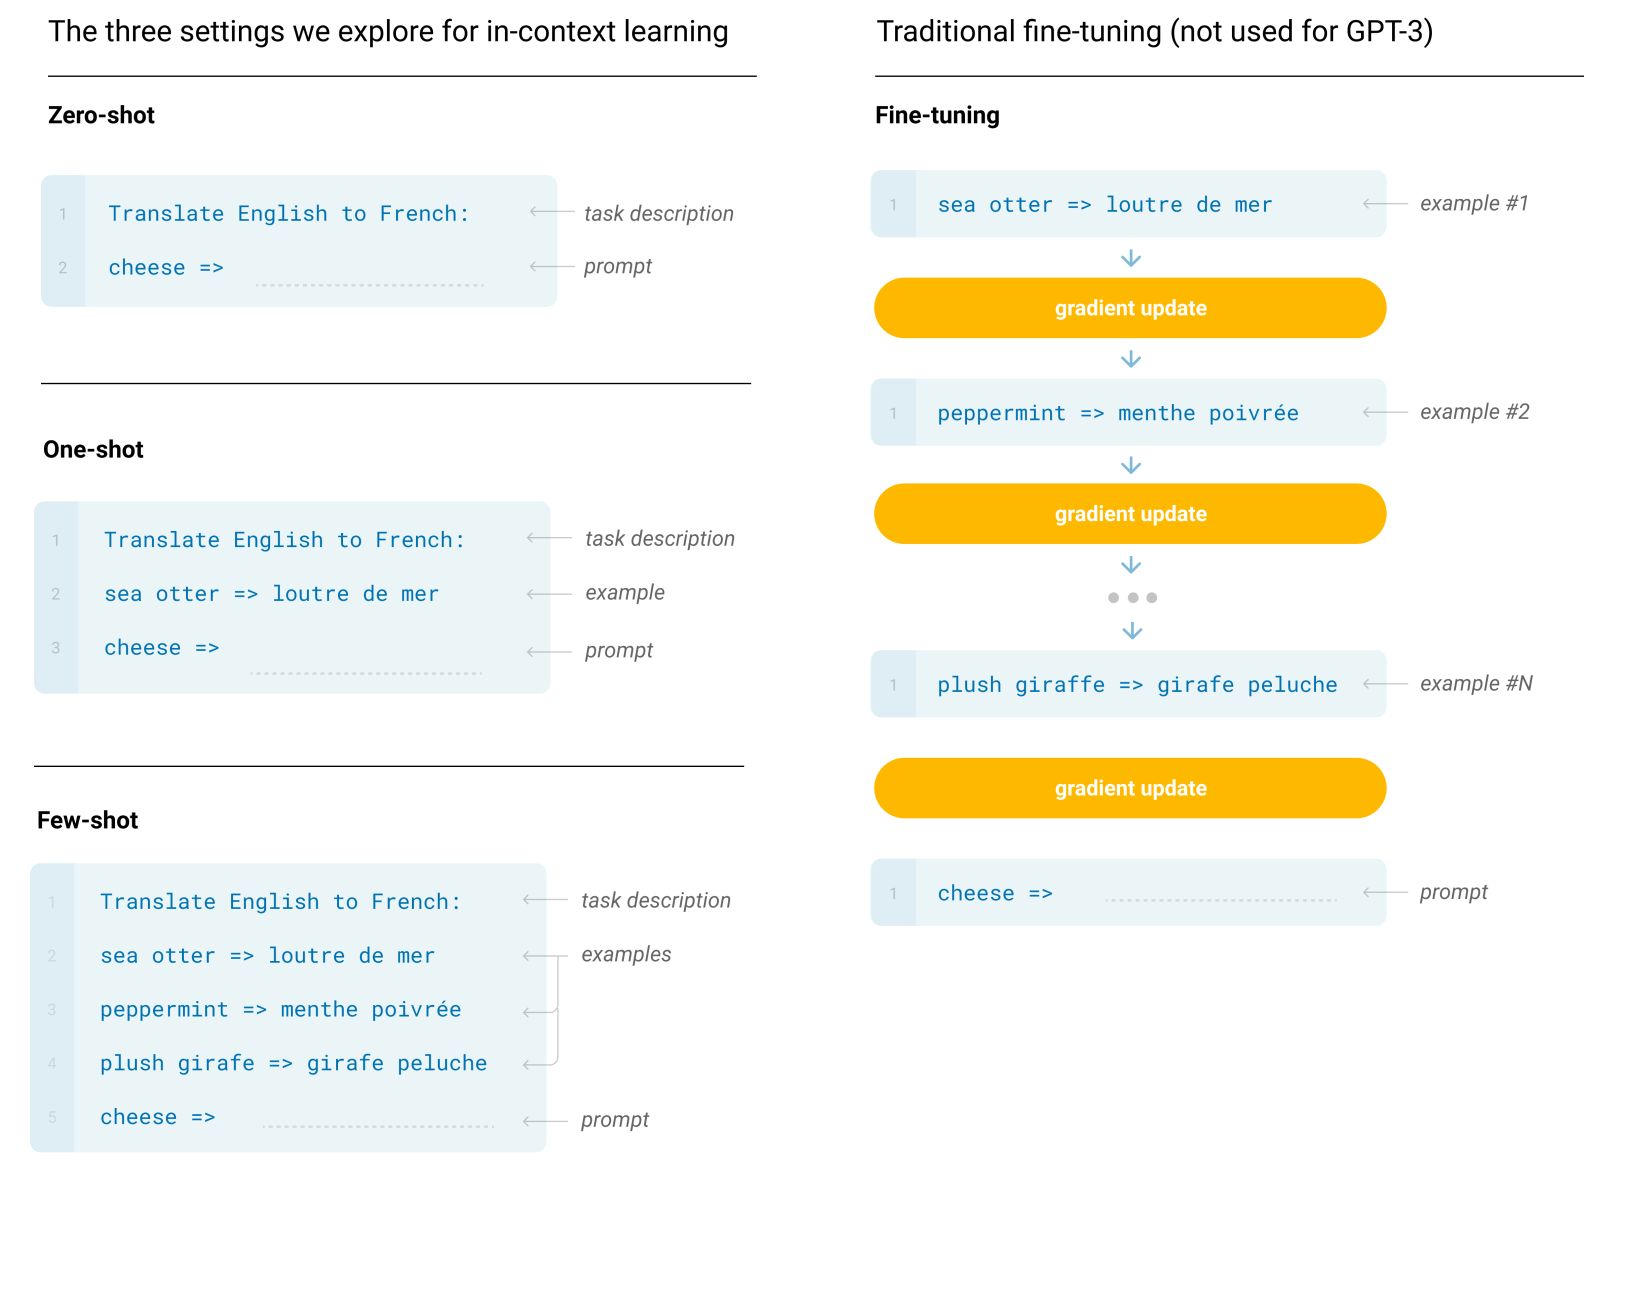
\includegraphics[scale = 0.12]{pics/zeroonefew.png}
        \end{figure}  

This means that they can learn new tasks without large amounts of human-annotated data.


\end{frame}


\begin{frame}{Talk Overview}
\begin{scriptsize}
\begin{itemize}
 \item Despite the recency of this technology, its adoption has been tremendous in many areas. 
 \item Below, we propose a simple categorization of the ways in which LLMs are used and evaluated.
  \item These patterns will serve as the narrative backbone of this presentation.
\end{itemize}



\begin{columns}[t]
\column{0.5\textwidth}
\begin{block}{Usage Patterns}
\begin{enumerate}
\item General-domain Assistant
\item Domain-specific Assistant
\begin{enumerate}\scriptsize
\item Retrieval-augmented generation
\item Fine-Tuning
\end{enumerate}
\item LLM-based Applications
\begin{enumerate}\scriptsize
\item API calls
\item Autonomous Agents
\end{enumerate}
\end{enumerate}
\end{block}

\column{0.5\textwidth}
\begin{block}{Evaluation Patterns}
\begin{itemize}
\item MTBench
\item LLM Arena
\end{itemize}
\end{block}

\end{columns}

\end{scriptsize}
\end{frame}









% \url{https://ai.meta.com/llama/get-started/?trk=feed_main-feed-card_reshare_feed-article-content}.

\section{General-domain Assistant}

\begin{frame}{Usage Pattern 1: General-domain Assistant}
\begin{scriptsize}
\begin{itemize}
\item In this pattern a user interacts with the LLM proving prompts as input and receiving a text as answer.
\item The knowledge the LLM has access is limited to the corpus on which it was trained and the context given in the prompt.
\end{itemize}

 \begin{figure}[h]
        	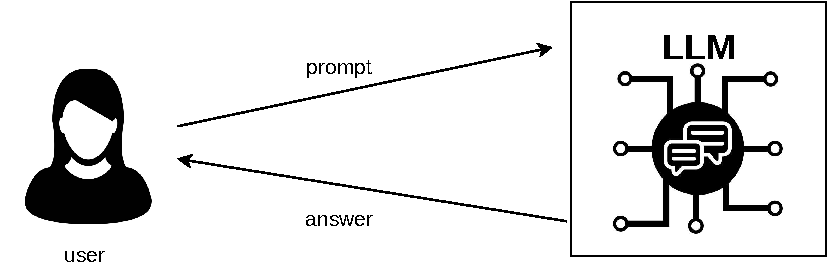
\includegraphics[scale = 0.6]{pics/assistantpattern.pdf}
        \end{figure}  


\end{scriptsize}
\end{frame}


\begin{frame}{Tasks}
\begin{scriptsize}
LLMs can solve many tasks with this pattern:

\begin{itemize}
\item Textual: Language understanding and common sense (e.g., rewriting, summarizing, translating, answering questions)
\item Arithmetic: Mathematical reasoning  (it can fail in many cases though)
\item Visual: Multimodal reasoning involving pictures (GPT-4, Llava)
\item Symbolic: Structured input such as programming languages
\end{itemize}
Source: \url{https://twitter.com/IntuitMachine/status/1727079666001870877}.
\end{scriptsize}
\end{frame}


\begin{frame}{Prompt Engineering: Guiding the Language Model}
\begin{scriptsize}
Prompt engineering, often referred to as ``Prompting,'' is the discipline or ``art'' of crafting effective prompts to guide the Language Model (LM) towards generating accurate responses. Some common prompting guidelines: \vspace{0.5cm}

\begin{itemize}
\item \textbf{Clarity and Conciseness}: Clearly articulate the prompt to minimize ambiguity and ensure the LM understands the task at hand.
\item \textbf{Use of Specific Examples}: Provide concrete examples within the prompt to offer the LM context.
\item \textbf{Role-based Prompts}: incorporating roles into the prompts (e.g., a tour guide, a teacher, a doctor, a sales person).
\item \textbf{Desired Output Specification}: Clearly define the desired format of the output (e.g, JSON, HTML, csv, markdown, latex).
\end{itemize}
\end{scriptsize}
\end{frame}


\begin{frame}{Chain-of-thought Prompting}

\begin{scriptsize}
\begin{itemize}
\item Chain-of-thought prompting is a simple mechanism for eliciting multi-step reasoning behavior in large language models.
\item  This method involves augmenting each exemplar in a few-shot prompt with a connected sequence of thoughts, creating a structured chain of logical steps. \cite{wei2022chain}
\end{itemize}
\end{scriptsize}



 \begin{figure}[h]
        	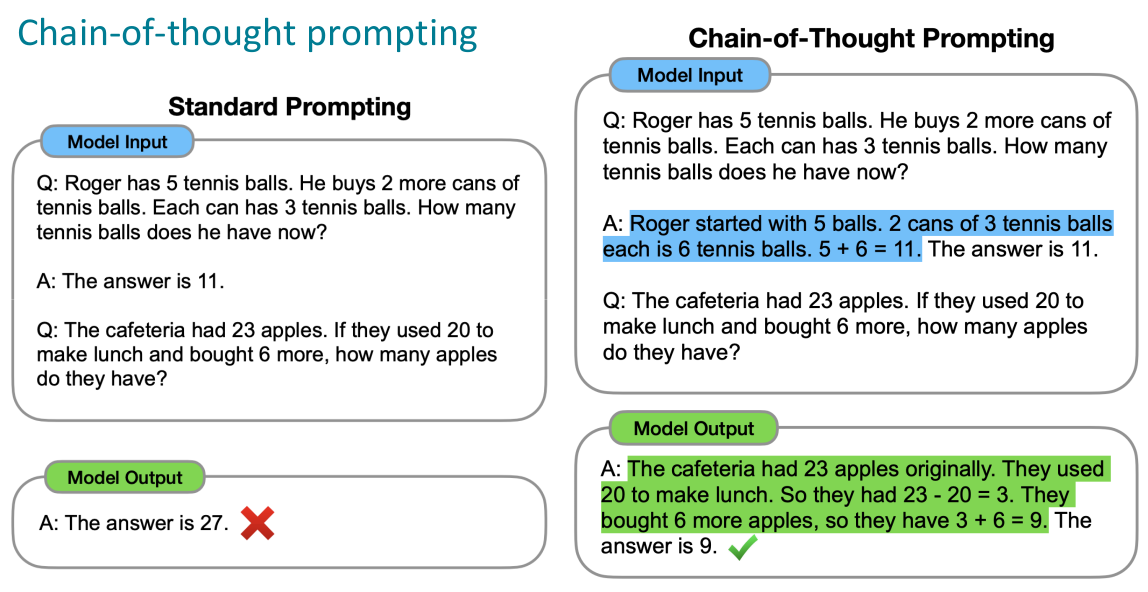
\includegraphics[scale = 0.3]{pics/chainoftought.png}
        \end{figure}



\end{frame}


\section{Domain-specific Assistant}

\begin{frame}{Usage Pattern 2: Domain-specific Assistant}
\begin{scriptsize}
\begin{itemize}
\item Idea: Incorporate domain-specific knowledge not covered in training (e.g., recent news, private documents).
\item This is very common for companies developing chatbots with private documents or for creating more domain-specific chatbots.
\item There are two main patterns to achieve this:
\begin{enumerate}\scriptsize
 \item Retrieval-Augmented Generation (Vector Databases)
 \item Fine-Tuning
\end{enumerate}
\end{itemize}


\end{scriptsize}
% https://platform.openai.com/docs/guides/fine-tuning/common-use-cases
\end{frame}


\begin{frame}{Usage Pattern 2.1: Retrieval-Augmented Generation}
\begin{scriptsize}
Idea: Incorporate domain-specific knowledge into the query using information retrieval and document embeddings (i.e., densely encoded vectors that capture the semantic information of the document). \cite{lewis2021retrievalaugmented}.

\end{scriptsize}

    \begin{figure}[h]
        	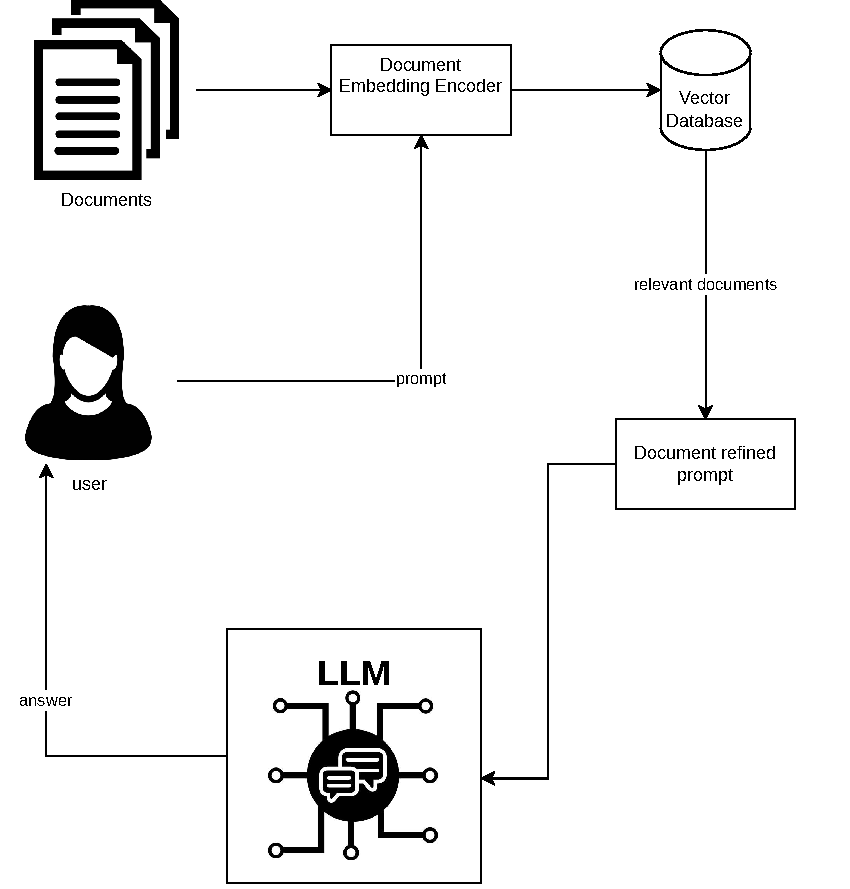
\includegraphics[scale = 0.4]{pics/retrievalaugmented.pdf}
        \end{figure}  


\end{frame}


\begin{frame}{Retrieval-Augmented Generation Process}
\begin{scriptsize}
\begin{enumerate}
 \item Encode all domain-specific documents using document embeddings and store them in a vector database.  
  \begin{itemize}\scriptsize
    \item OpenAI provides a vectorizer called (text2vec-openai), but there are many open source alternatives.
 \item There are also many vector databases available, a popular one is \textbf{weaviate}.
  \end{itemize}
 \item Encode the prompt with the same vectorizer used to encode documents.
 \item Use prompt embedding and the vector database to retrieve relevant documents based on similarity.
 \item Create a refined prompt that includes a domain-specific role, the user prompt, and the retrieved documents as contexts.
 \item Send the refined prompt to the LLM and return the response to the user.
\end{enumerate}

\end{scriptsize}



\end{frame}

 

%\item \url{https://www.infoworld.com/article/3709912/vector-databases-in-llms-and-search.html}
%\item \url{https://learn.deeplearning.ai/vector-databases-embeddings-applications/lesson/1/introduction}
%\item \url{https://stackoverflow.blog/2023/10/09/from-prototype-to-production-vector-databases-in-generative-ai-applications/}


\begin{frame}{Usage Pattern 2.2: Fine-Tuning}
\begin{scriptsize}
Idea: Incorporate domain-specific knowledge by fine-tuning a pre-trained LLM with the next-token prediction task over a domain-specific corpus and interact with the resulting LLM. 



    \begin{figure}[h]
        	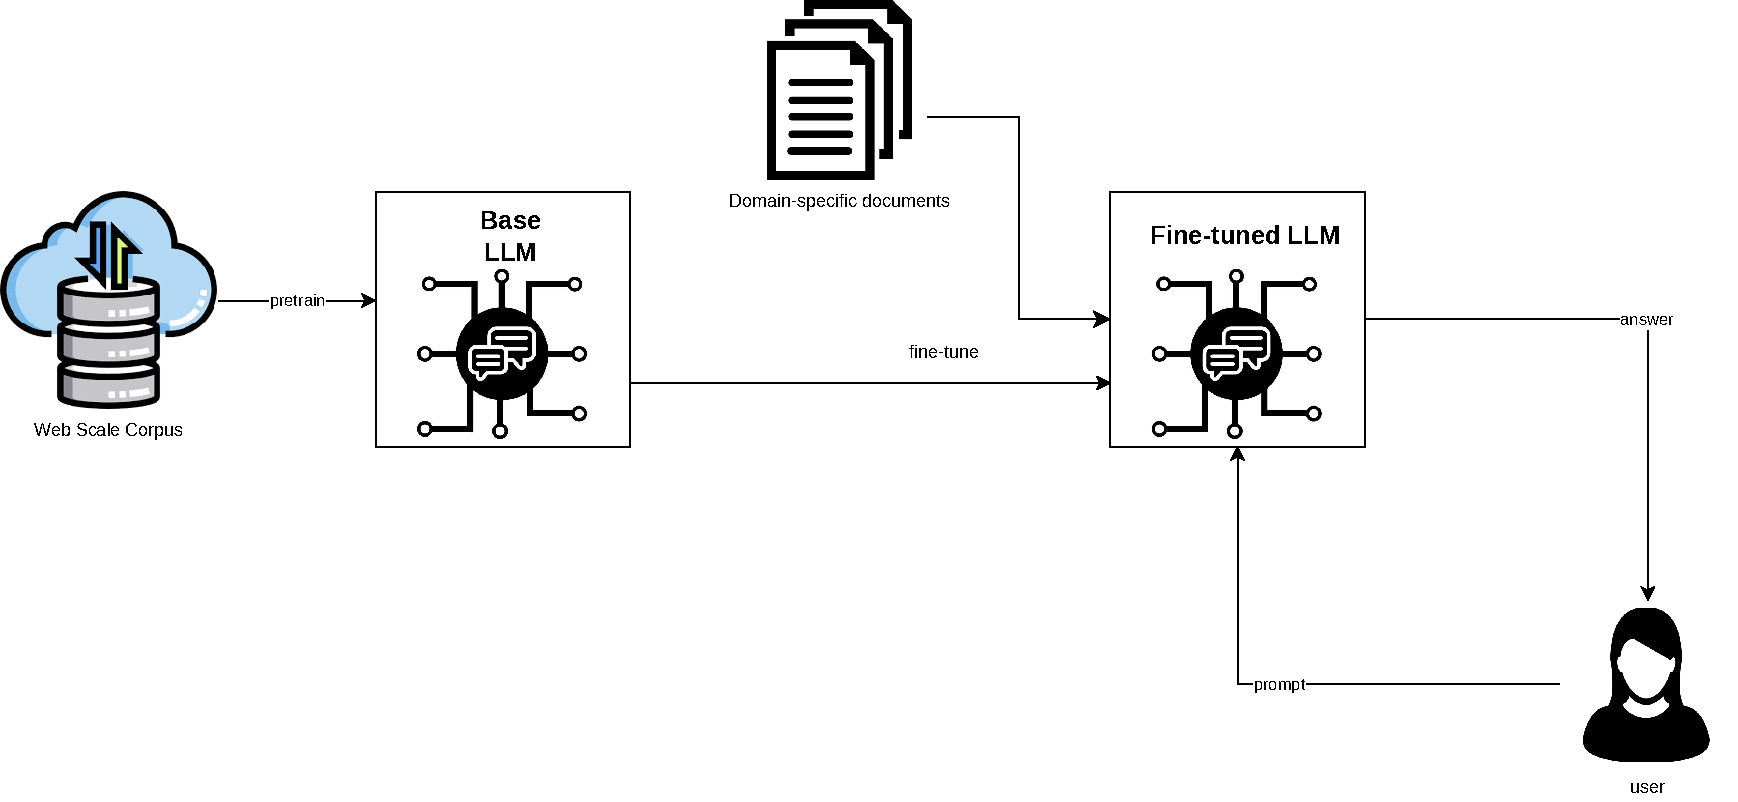
\includegraphics[scale = 0.35]{pics/llmfinetuning.pdf}
        \end{figure}  

This can be computationally expensive unless some tricks are used.
\end{scriptsize}
\end{frame}


\begin{frame}{Instruction Fine-tuning}

\begin{scriptsize}
\begin{itemize}
\item A more efficient way to fine-tune Large Language Models is Instruction Fine-Tuning  \cite{chung2022scaling}.
\item Idea: instead of fine-tuning the LLM with raw text with next token prediction, train it with pairs of prompts and user-aligned answers.
\item Collect examples of (instruction, output) pairs across many tasks and finetune an LM.
\item Evaluate on unseen tasks.
\end{itemize}

\begin{figure}[h]
	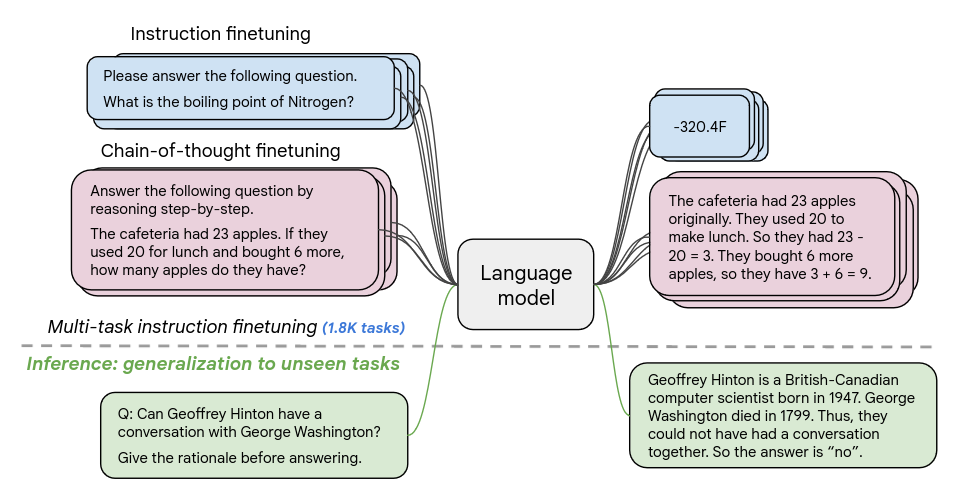
\includegraphics[scale = 0.35]{pics/instructionfinetuning.png}
\end{figure}


\end{scriptsize}






\end{frame}


%\begin{frame}{Instruction Fine-Tuning}

%Setting the style, tone, format, or other qualitative aspects, Improving reliability at producing a desired output Correcting failures to follow complex prompts   Handling many edge cases in specific ways     Performing a new skill or task that’s hard to articulate in a prompt

% https://nlpnewsletter.substack.com/p/instruction-tuning-vol-1

%\begin{scriptsize}
%\begin{itemize}
%\item Paid Fine-Tuning (GPT-4??)
%\item OpenAI offers many more specific gpts: \url{https://openai.com/blog/%introducing-gpts}
%\item Alpaca, Vicuna, Llama, Llama2
%\item https://blog.gopenai.com/paper-review-qlora-efficient-finetuning-of-%quantized-llms-a3c857cd0cca
%\end{itemize}
%\end{scriptsize}
%\end{frame}

\begin{frame}{Datasets for Instruction Fine-Tuning}
\begin{scriptsize}
\begin{itemize}
\item Alpaca Data: 52k English instruction examples generated using OpenAI’s text-davinci-003 with self-instruct.
\item Evol-Instruct (Xu et al., April 2023): A rewritten set of 250k English instruction-response pairs based on the Alpaca data
\item Vicuna ShareGPT: 70k English conversations shared by users and scraped from \item Baize data (Xu et al., April 2023)
\item databricks-dolly-15k (Conover et al., April 2023)
\item OpenAssistant Conversations (Köpf et al., April 2023)
\item LIMA data (Zhou et al., May 2023).
\end{itemize}
source: \url{https://nlpnewsletter.substack.com/p/instruction-tuning-vol-2}
\end{scriptsize}
\end{frame}

% Self-instruct https://arxiv.org/pdf/2212.10560.pdf

\begin{frame}{Considerations for Instruction Tuning}
\scriptsize


\begin{itemize}
    \item \textbf{Data Source:} How was the data obtained? Most datasets have been generated using ChatGPT. They may thus inherit biases of the source model or may be noisy.

    \item \textbf{Data Quality:} Was any filtering done to improve the quality of the generated data? In most cases, filtering is based on simple heuristics or a pre-trained model, which can result in noisy data.

    \item \textbf{Domain and Language Coverage:} Most datasets focus on general QA-style in English, but methods can be adapted for other domains or languages.

    \item \textbf{Number of Dialog Turns:} Single-turn datasets include a prompt and response. Consider multi-turn data for training a more conversational model.

    \item \textbf{License Terms:} Data from OpenAI models follows OpenAI terms, restricting use for competing models. Seek datasets with more permissive licenses to avoid legal complications.
\end{itemize}
source: \url{https://nlpnewsletter.substack.com/p/instruction-tuning-vol-2}
\end{frame}



%LoRA is an improved finetuning method where instead of finetuning all the weights that constitute the weight matrix of the pre-trained large language model, two smaller matrices that approximate this larger matrix are fine-tuned. These matrices constitute the LoRA adapter. This fine-tuned adapter is then loaded to the pretrained model and used for inference.

%QLoRA is an even more memory efficient version of LoRA where the pretrained model is loaded to GPU memory as quantized 4-bit weights (compared to 8-bits in the case of LoRA), while preserving similar effectiveness to LoRA. Probing this method, comparing the two methods when necessary, and figuring out the best combination of QLoRA hyperparameters to achieve optimal performance with the quickest training time will be the focus here.

% Token-Incrementation



\begin{frame}{Parameter Efficient Fine Tuning (PEFT)}
\begin{scriptsize}
\begin{itemize}
    \item Traditional model fine-tuning (i.e., adjusting all Transformer weights via backpropagation) is time and resource-intensive.
    \item Parameter Efficient Fine Tuning (PEFT) are a series of techniques to mitigate this problem.
    \item The most popular ones are LoRA (Low Rank Adaptation) \cite{hu2021lora} and QLoRA \cite{dettmers2023qlora}.
    \item These approaches achieve siginficant reduction in the number of trainable parameters allowing to perform fine-tuning with affordable hardware.
\end{itemize}
\end{scriptsize}
\end{frame}


\begin{frame}{LoRA}
\begin{scriptsize}
\begin{itemize}
    \item LoRa is based on the idea of adapters.
\item Instead of fine-tuning the whole network, we freeze it during the fine-tuning process and add a few parameters that are trained to adapt the original model to the new data.
          \end{itemize}

      \begin{figure}[h]
	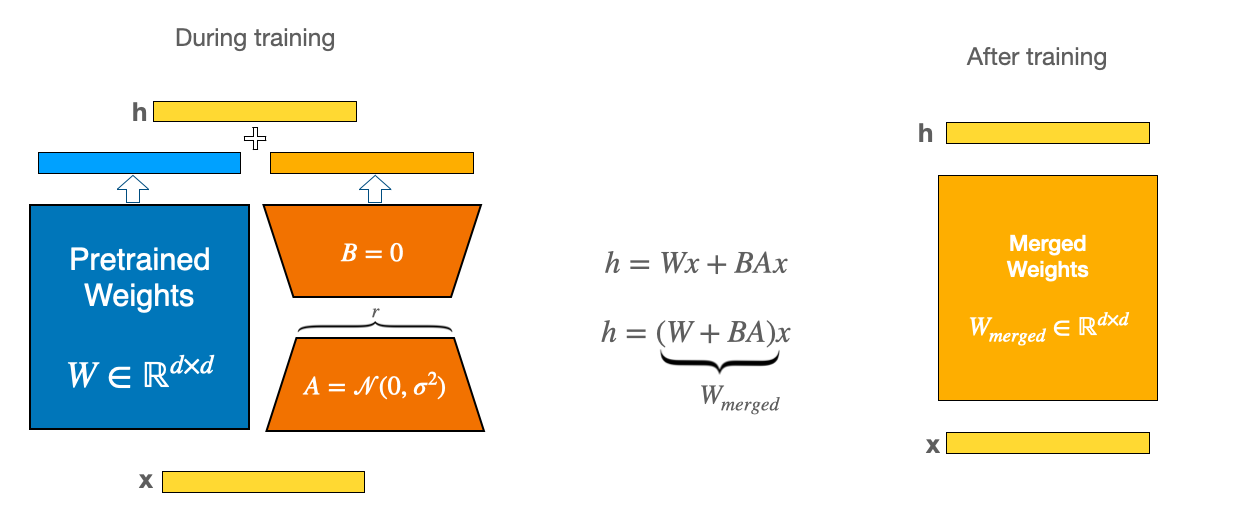
\includegraphics[scale = 0.35]{pics/lora.png}
\end{figure}

\end{scriptsize}
\end{frame}


\begin{frame}{LoRA}
\begin{scriptsize}
\begin{itemize}
        \item Let $W_0 \in \mathbb{R}^{d \times k}$ be the weight matrix of the pre-trained network.
    \item LoRA uses two adjustable low-rank decomposition matrices of predefined rank $r$, \(B \in \mathbb{R}^{d \times r}\) and \(A \in \mathbb{R}^{r \times k}\).
    \item The resulting fine-tuned network $W_L$ is obtained as follows:
      \begin{equation}
    W_L = W_0 + \Delta W = W_0 + BA, \quad B \in \mathbb{R}^{d \times r}, \quad A \in \mathbb{R}^{r \times d}
  \end{equation}
 \item During training, \(W_0\) remains frozen, and only \(B\) and \(A\) receive gradient updates.
 \item The lower the value of $r$, the fewer parameters will be trained during fine-tuning (there is a trade-off between performance and computation costs).
      \end{itemize}

\end{scriptsize}
\end{frame}

\begin{frame}{QLoRA}
\begin{scriptsize}
\begin{itemize}
\item QLoRA is an even more memory efficient version of LoRA where the pretrained model is loaded to GPU memory as \textbf{quantized} 4-bit weights.
\item QLoRA dequantizes weights from the storage data type to the computation data type to perform the forward and backward passes.
\item It only computes weight gradients for the LoRA parameters which use 16-bit bfloat.
\item QLORA reduces the average memory requirements of finetuning a 65B parameter model from $>780GB$ of GPU memory to $<48GB$.
\end{itemize}
\end{scriptsize}
     \begin{figure}[h]
	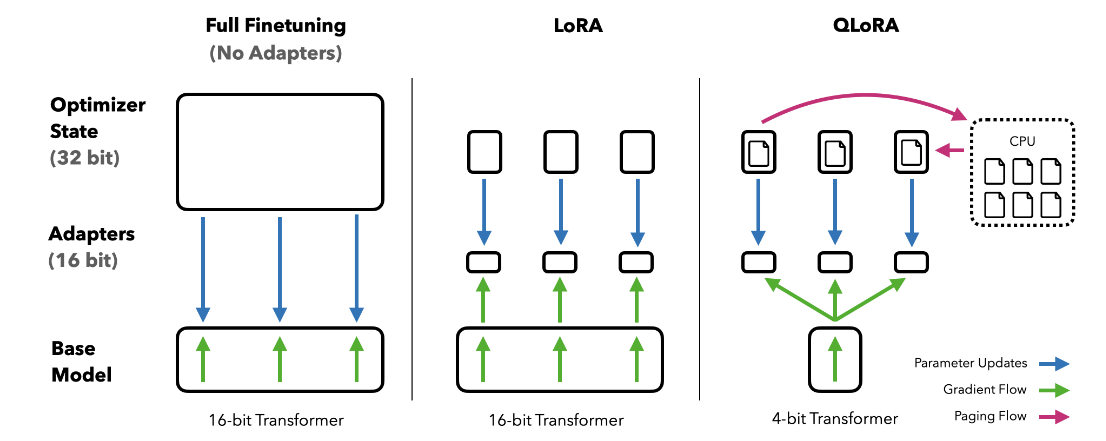
\includegraphics[scale = 0.22]{pics/qlora.png}
\end{figure}

\end{frame}

\begin{frame}{Quantization}
\scriptsize
    \begin{itemize}
        \item Quantization: Process of discretizing input from high-bit representation to low-bit representation.
      \item To ensure that the entire range of the low-bit data type is used, the input data type is commonly rescaled into the target data type range through normalization by the absolute maximum of the input elements.
        \item Example: quantizing a 32-bit Floating Point (FP32) tensor into a Int8 tensor with range $[-127, 127]$:
        \[X_{\text{Int8}} = \text{round}_{\text{digits}(0)}\left(\frac{127}{\text{absmax}(X_{\text{FP32}})} \cdot X_{\text{FP32}}\right) = \text{round}_{\text{digits}(0)}\left(c_{\text{FP32}} \cdot X_{\text{FP32}}\right)\]
        where $c$ is the quantization constant or quantization scale.
        \item Dequantization:
    \[\text{dequant}(c_{\text{FP32}}, X_{\text{Int8}}) = \frac{X_{\text{Int8}}}{ c_{\text{FP32}}} = X_{\text{FP32}}\]
    \end{itemize}
\end{frame}

\begin{frame}{Quantization}
     \begin{figure}[h]
	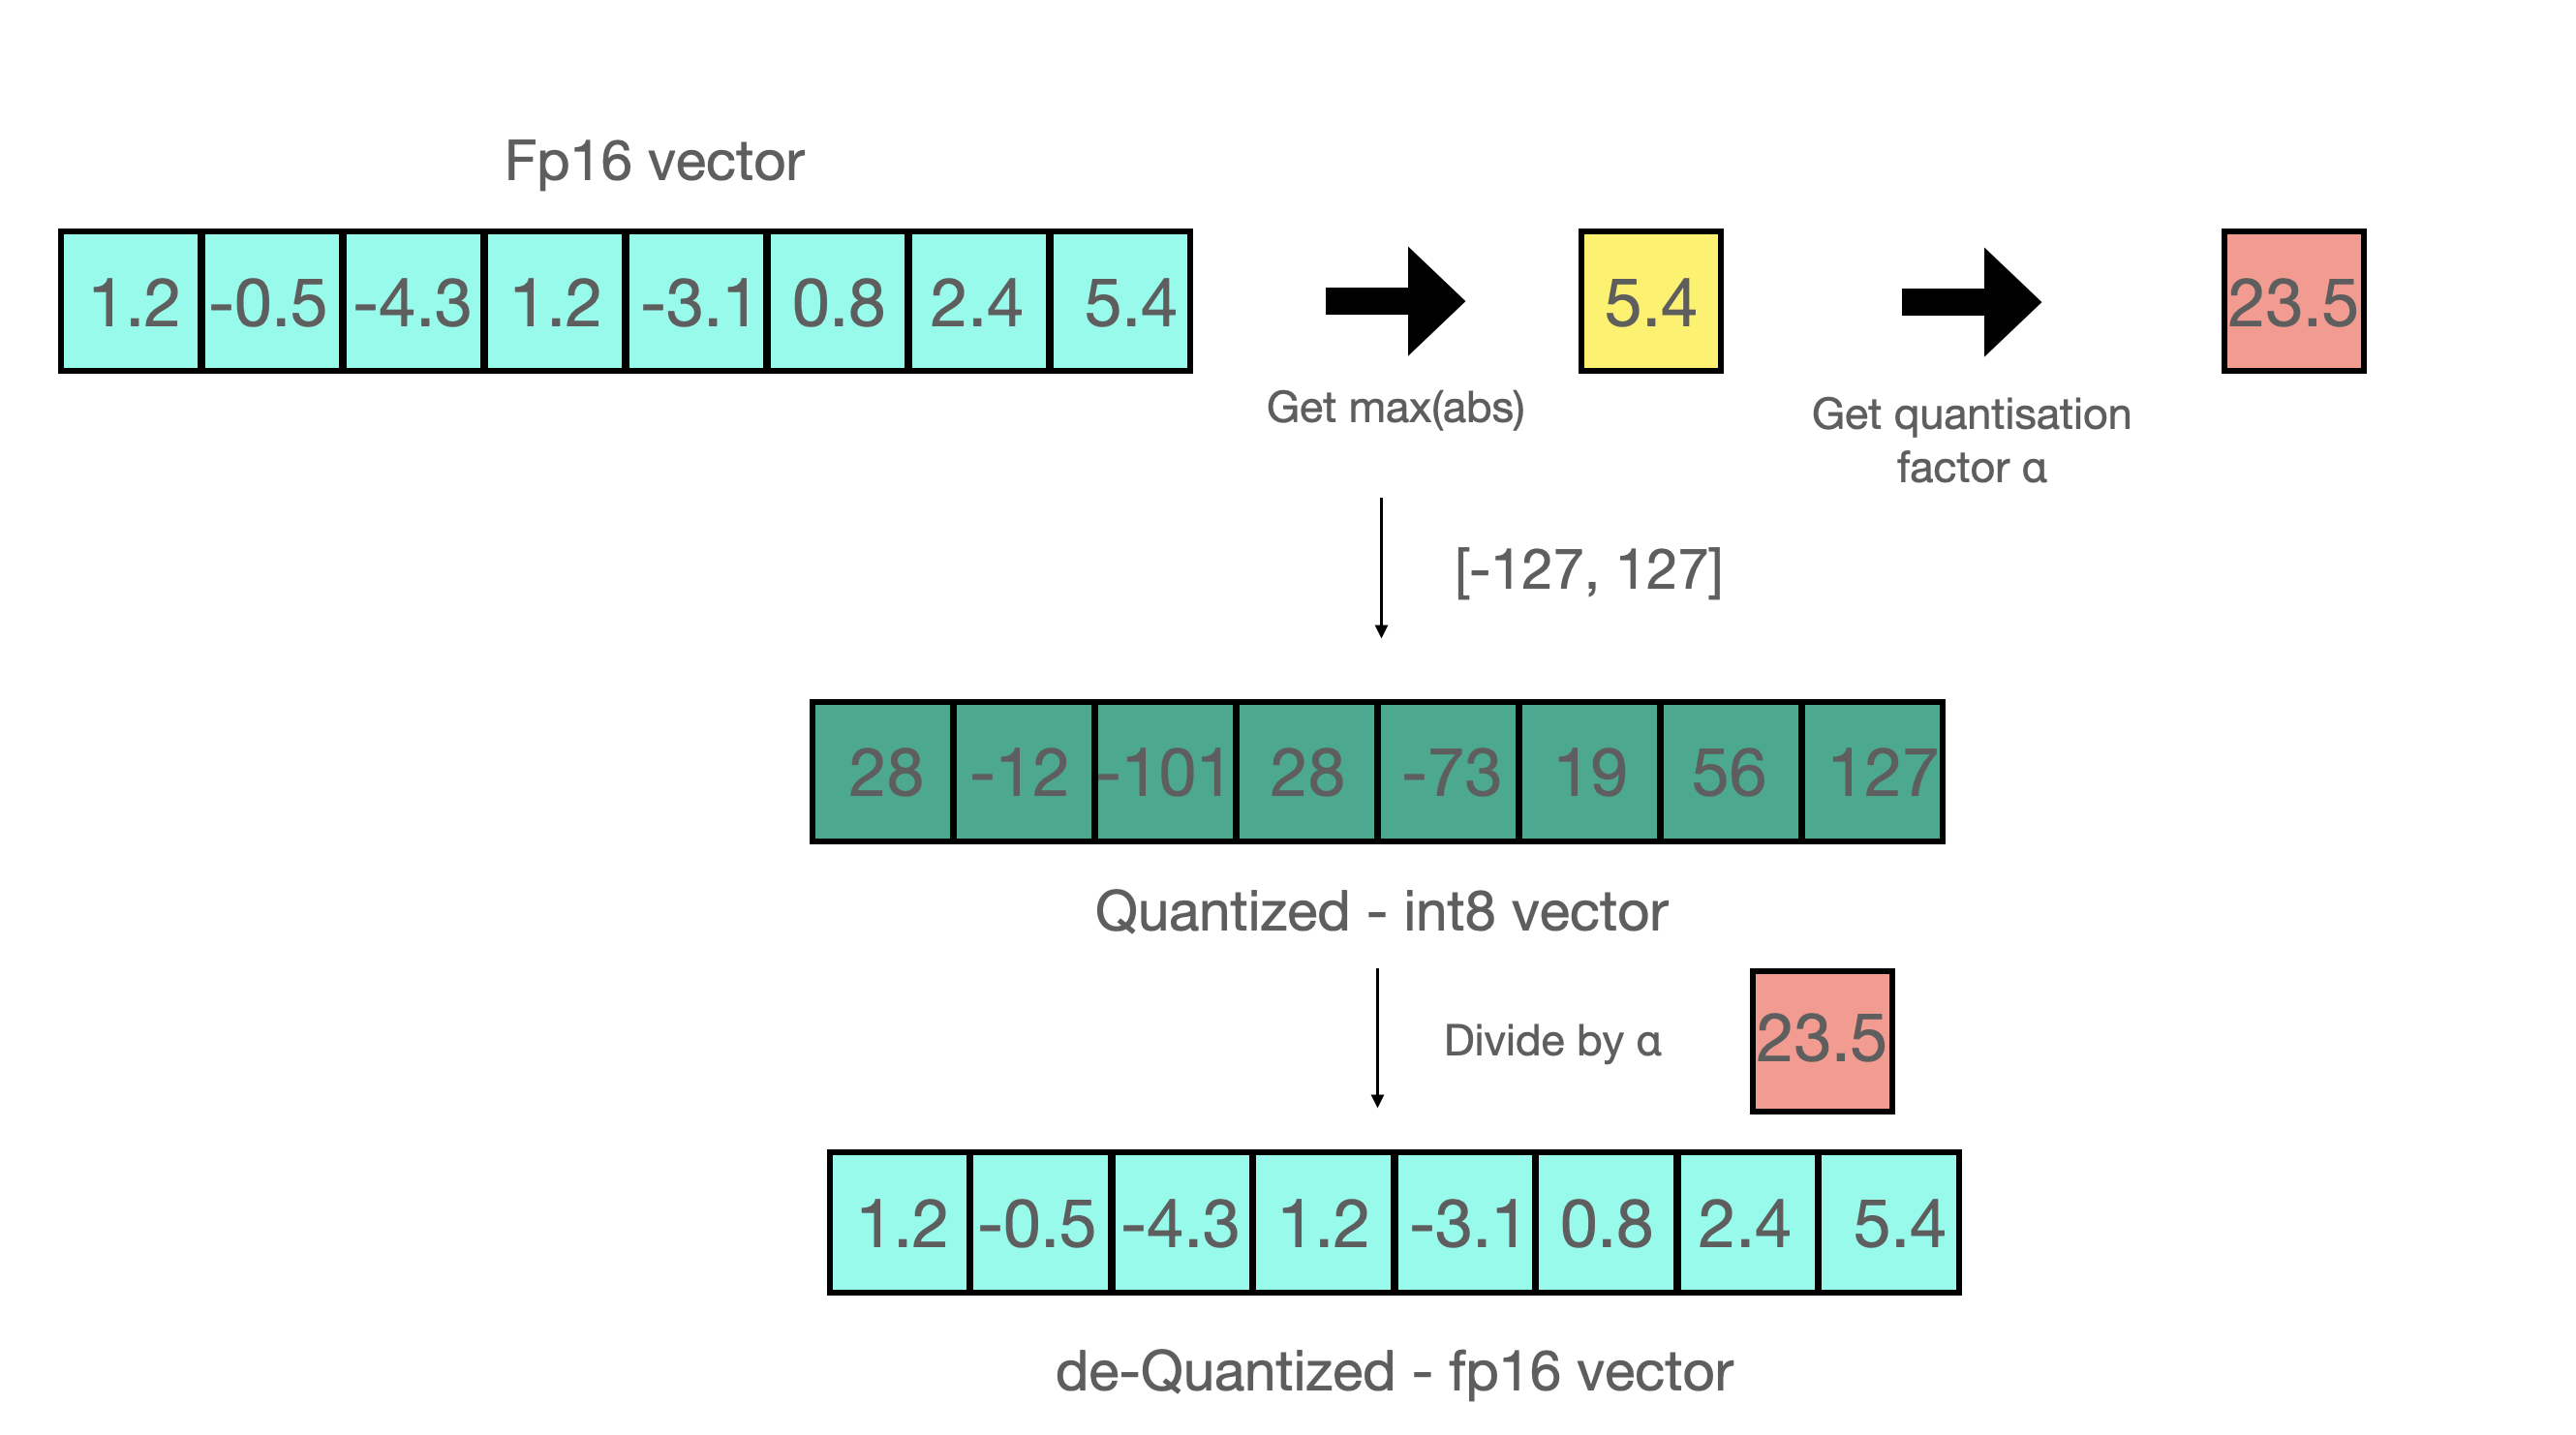
\includegraphics[scale = 0.22]{pics/quant-freeze.png}
\end{figure}
source: \url{https://huggingface.co/blog/hf-bitsandbytes-integration}
\end{frame}


\begin{frame}{QLoRA main Ideas}
\begin{scriptsize}
\begin{itemize}
\item  4-bit NormalFloat, an information theoretically optimal quantization data type for normally distributed data\footnote{pretrained neural network weights usually have a zero-centered normal distribution with standard deviation $\sigma$}  that yields better empirical results than 4-bit Integers and 4-bit Floats.
\item Double Quantization, a method that quantizes the quantization constants, saving an average of about 0.37 bits per parameter (approximately 3 GB for a 65B model).
\item Paged Optimizers, using NVIDIA unified memory to avoid the gradient checkpointing memory spikes that occur when processing a mini-batch with a long sequence length.
\end{itemize}
\end{scriptsize}

\end{frame}



\section{Applications}

\begin{frame}{Usage Pattern 3: Applications}
\begin{scriptsize}
\begin{itemize}
\item LLMs are widely embedded in software through API calls.
\item Example: search engines (\url{you.com}), Bing chat.
\item For example, PDF summarization software. You write software that first converts the PDF to raw text and then sends it to an LLM for summarization.
\item Or software for summarizing video conferences. First the audio is transcribed and then summarized with an LLM.
\item From a software point of view, this isn't much different from any software that interacts with an external API.
\item ChatGPT Plugins: \url{https://gptstore.ai/}
\end{itemize}
\end{scriptsize}
\end{frame}


\begin{frame}{Usage Pattern 3: Applications}

      \begin{figure}[h]
	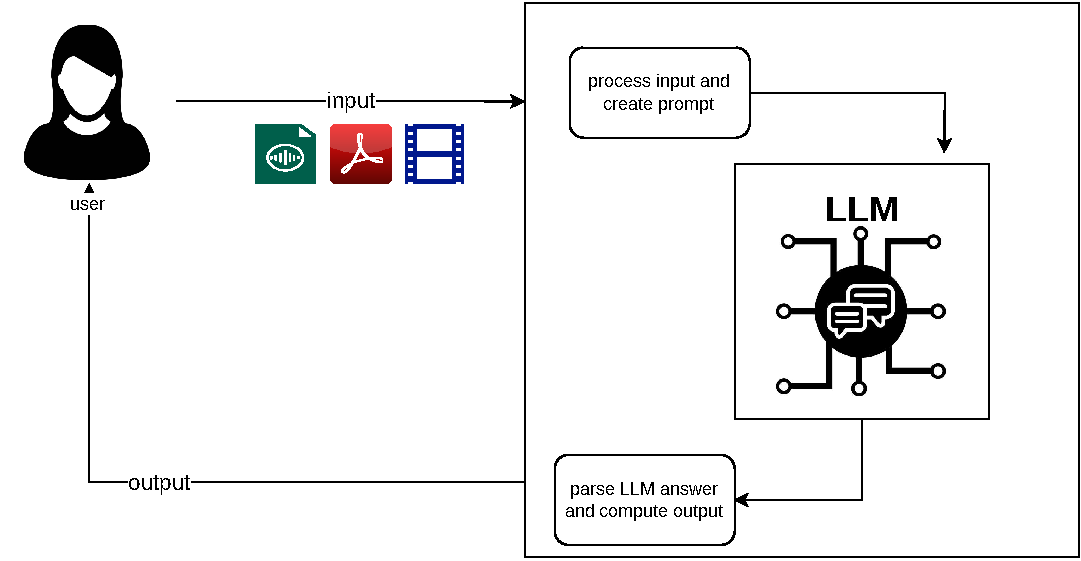
\includegraphics[scale = 0.55]{pics/llmsapp.pdf}
\end{figure}

\end{frame}


\begin{frame}{Usage Pattern 3.1: Autonomous Agents}
%https://arxiv.org/pdf/2304.03442.pdf
% https://arxiv.org/abs/2210.03629
%https://bootcamp.uxdesign.cc/a-comprehensive-and-hands-on-guide-to-autonomous-agents-with-gpt-b58d54724d50
% https://leftasexercise.com/2023/06/17/autonomous-agents-and-llms-autogpt-langchain-and-all-that/
\begin{scriptsize}
\begin{itemize}
\item Autonomous agents lie at the heart of classical AI.
\item Agents are programs that interact autonomously with an environment and perform actions to achieve specific goals.
\item The REACT pattern \cite{yao2022react} aims uses LLMs to generate both reasoning traces and task-specific actions in an interleaved manner for agents.


\item Agents are a special kind of LLMs application in which the LLM serves as the reasoning and planning component of the software.
\end{itemize}
\end{scriptsize}
\end{frame}


\begin{frame}{Agents}
\scriptsize
    \begin{itemize}
        \item General setup: Agent interacting with an environment.
        \item At time step $t$, agent receives observation $o_t \in O$ and  takes action $a_t \in A$ following policy $\pi(a_t | c_t)$ where context $c_t = (o_1, a_1, \ldots, o_{t-1}, a_{t-1}, o_t)$.
        \item Implicit mapping $c_t \mapsto a_t$ with extensive computation.
        \item Example: Agent in Figure 1(1c) unable to generate correct final action (Act 4).
        \item Example: Agent in Figure 1(2a) fails to comprehend context, producing hallucinating actions.
    \end{itemize}
\end{frame}

\begin{frame}{The ReAct Approach}
\scriptsize
\begin{itemize}
        \item Augment agent's action space: $\hat{A} = A \cup L$, where $L$ is the language space.
        \item $\hat{a}_t \in L$ is a thought or reasoning trace, not affecting the environment.
        \item Thought aims to compose useful information by reasoning over the context $c_t$.
        \item Update context: $c_{t+1} = (c_t, \hat{a}_t)$ for future reasoning or acting.
        \item Decomposing task goals and creating action plans (2b, Act 1; 1d, Thought 1).
        \item Injecting commonsense knowledge relevant to task solving (2b, Act 1).
        \item Extracting important parts from observations (1d, Thought 2, 4).
        \item Tracking progress and transiting action plans (2b, Act 8).
        \item Handling exceptions and adjusting action plans (1d, Thought 3).
    \end{itemize}
\end{frame}

% Patterms can be combined: Gorilla, LLama2 fine-tuned to be good at API calls and then used in agents.


\section{Evaluation Patterns}
\begin{frame}{LLMBench and LLm Arena}
\begin{scriptsize}
\begin{itemize}
\item Standard NLP evaluation: human annotated gold-labels and metrics.
\item LLMS are intrinsically multi-task and not easily evaluated with this approach.
\item Machines evaluating machines??
\item MT-bench (categories)
\item HuggingFace Open LLM Leaderboard
\item LLM Arena
\end{itemize}
\end{scriptsize}
\end{frame}

\begin{frame}
\frametitle{Questions?}
%\vspace{1.5cm}
\begin{center}\LARGE Thanks for your Attention!\\ \end{center}



\end{frame}

\begin{frame}[allowframebreaks]\scriptsize
\frametitle{References}
\bibliography{bio}
\bibliographystyle{apalike}
%\bibliographystyle{flexbib}
\end{frame}  


%%%%%%%%%%%%%%%%%%%%%%%%%%%

\end{document}
